\section{Results for modified gravity}
In this section we apply the approximate techniques to chameleon gravity. Parameters of all run and analyzed simulations are described in \autoref{tab:cham_param_CHI_lin} and \autoref{tab:cham_param_CHI_nl}. We focused on issues closely related to the scale where the chameleon field starts to affect the matter distribution. We first wish to study the effects of varying the simulation resolution on the power spectrum. Because the screening mechanism is directly related to the depth of the gravitational wells, and with lower spatial resolution, these wells are smeared, the role of resolution also needs to be understood. For this analysis we chose the FPA as this approximation is closest in spirit to \nbodysim s.

Following this, we compare the results of chameleon gravity directly against the FPA and FFA simulations. %These comparisons can tell us a lot about when and on what scales are chameleon effects visible and which approximation is better for studying modified gravity. 
We will study both $k-$space effects (power spectrum) and real-space effects (BAO peak in the correlation function). For chameleon gravity we ran all simulations twice -- once solving the non-linear Poisson equation \eqref{eq:cham_u_cp} using the multigrid solver, and the second using the pseudo-linear prediction for the chameleon in $k-$space given by \eqref{eq:chi_lin_k_cp} corrected by \eqref{eq:chi_bulk_cp}.

%%%%%%%%%%%%%%%%%%%%%%%%%%%%%%%%%%%%%%%%
% Effect of simulation resolution
%%%%%%%%%%%%%%%%%%%%%%%%%%%%%%%%%%%%%%%%
\subsection{Effect of simulation resolution}
In order to study the effects of the simulation resolution, we define this resolution via the Nyquist wave-number $\knq$
\eq{
\knq=\frac{\pi N_f}{L}\,.
}
We wish to study two things in particular. The first is the minimum resolution needed to explore some particular scale, i.e., whether non-linear effects on smaller scales can affect larger scales. The second is to study the validity range of the pseudo-linear approximation of the chameleon field. We want to investigate on which scale this approximation breaks down and cannot be used even for generating approximate results.

In \autoref{fig:chi_res}, we see several chameleon simulations $(n=0.5,\ \Phiscr=10^{-5})$ with different resolution. We compared the resulting power spectra directly with FPA simulations with the same parameters (box size, number of particles, etc.). There are four sets of simulations with different resolutions (Nyquist frequencies), each one with a pseudo-linear prediction for the chameleon field and a non-linear result from the multigrid solver.

For lower resolution $(\knq = 0.4~\hMpc$ and $\knq = 0.8~\hMpc$), the pseudo-linear theory predicts higher amplitude of the power spectrum as it underestimates the screening effect on smaller scales. However, with higher resolution (and the ability to see deeper gravitational wells) this pseudo-linear prediction starts to overestimate the screening and suppress the power spectrum sooner than in the non-linear solver. It is because the correction to the solution \eqref{eq:chi_lin_k_cp} suppress the chameleon force completely -- not only inside massive objects but near those as well. The non-linear solution predicts suppressed forces nearby these massive objects but not completely. The exact scale when this happens is dependent on the screening potential -- lower $\Phiscr$ means we need finer resolution to see deep gravitational wells where the chameleon is in the screening regime. For the choice of the screening potential as in \autoref{fig:chi_res} $(\Phiscr=10^{-5})$ this crossover where we cannot use the linear prediction happens at $k\sim2~\hMpc$. However, as FPA cannot fully resolve non-linear features on scales $k\gtrsim1~\hMpc$  we cannot take this scale exactly.

We can also see that even with higher resolution the power spectra on large and medium scales remain the same. This may suggest that the non-linear effects due to coupling of different wave-numbers are small. However, as these results are coming from a quasi-linear approximation we should be cautious about such a statement. We will further explore this resolution effects of the chameleon gravity using full \nbody s in the future.

\begin{figure}
  \centering
	\begin{subfigure}{1.0\textwidth}
        \includegraphicscustomlegend{simulations_approx/chi/chi_resolution_eff}
	\end{subfigure}
	\begin{subfigure}{1.0\textwidth}
		\includegraphicscustom{simulations_approx/chi/chi_resolution_eff}
	\end{subfigure}
  \caption{Ratio of the power spectrum of chameleon gravity to FPA with different resolutions of simulations. All simulations have $n=0.5,\ \Phiscr=10^{-5}$. Dotted lines show pseudo-linear prediction of the chameleon field whereas solid lines show results for the full non-linear multigrid solver for the chameleon field. Dashed vertical lines show locations of corresponding Nyquist frequencies.}
  \label{fig:chi_res}
\end{figure}

%%%%%%%%%%%%%%%%%%%%%%%%%%%%%%%%%%%%%%%%
% Matter power spectrum
%%%%%%%%%%%%%%%%%%%%%%%%%%%%%%%%%%%%%%%%
\subsection{Matter power spectrum}
We now turn to results for the matter power spectrum; \autoref{fig:pwr_spec_chi_fp} shows power spectra for different chameleon parameters for modified gravity simulations with FFA and FPA.

The FFA predicts an increased enhancement of the power spectrum compared to the FPA, unlike the corresponding situation for $\Lambda$CDM. This can be understood from how dynamics is treated within the FFA. In case of standard gravity, the velocity of a particle decreases steadily as it approaches a minimum of the gravitational potential. In the case of chameleon gravity, however, once the particle is close enough to the potential minimum such that the screening effect kicks in, the fifth force is abruptly cut off and the particle stops at the potential minimum. In the case of FPA, the particles retain their velocities inside the screened regions and the clustering effect, therefore, is not as strong.

\begin{figure*}
\centering
	\begin{subfigure}{1.2\textwidth}
        \includegraphicscustomlegend{simulations_approx/chi/fp_pwr_spec}
	\end{subfigure}
	\begin{subfigure}{0.5\textwidth}
		\includegraphicscustom{simulations_approx/chi/fp_pwr_spec}
	\end{subfigure}%
	\begin{subfigure}{0.5\textwidth}
		\includegraphicscustom{simulations_approx/chi/ff_pwr_spec}
	\end{subfigure}
	\begin{subfigure}{0.5\textwidth}
		\includegraphicscustom{simulations_approx/chi/fp_pwr_spec_ratio_nl}
	\end{subfigure}%
	\begin{subfigure}{0.5\textwidth}
		\includegraphicscustom{simulations_approx/chi/ff_pwr_spec_ratio_nl}
	\end{subfigure}
    \caption{Matter power spectrum $P(k)$ at redshift $z=0$ for different chameleon parameters. On the left are results using FPA whereas on the right results using FFA. Grey areas represent variations across different runs. Higher screening potential leads to greater enhancement of the power spectrum due to the fifth force.}
    \label{fig:pwr_spec_chi_fp}
\end{figure*}

In \autoref{fig:CHI_FP_diff}, we compare simulations with different chameleon parameters directly with FPA and FFA. For the values of the chosen screening potential $(\Phiscr=10^{-6}, 10^{-5}, 10^{-4})$ and a given resolution, the pseudo-linear prediction slightly underestimates the screening effect. The dependence of the enhancement of the power spectrum on chameleon parameters is according to our expectations. A lower value of the screening potential leads to a shorter Compton wavelength and greater effect of screening and therefore lower enhancement. Lower value of the chameleon power-law exponent leads to a longer Compton wavelength and higher screening potential $\Phiscra$ and therefore greater enhancement. We also again see that FFA predicts greater enhancement than FPA.

\begin{figure*}
  \centering
	\begin{subfigure}{1.2\textwidth}
        \includegraphicscustomlegend{simulations_approx/chi/chi_pwr_diff_256m_1p_512M_2000b}
	\end{subfigure}
	\begin{subfigure}{0.5\textwidth}
		\includegraphicscustom{simulations_approx/chi/chi_pwr_diff_256m_1p_512M_2000b}
	\end{subfigure}%
	\begin{subfigure}{0.5\textwidth}
		\includegraphicscustom{simulations_approx/chi/chi_ff_pwr_diff_256m_1p_512M_2000b}
	\end{subfigure}
  \caption{Ratio of the power spectrum of chameleon gravity to FPA (left) and FFA (right) with different chameleon parameters. Dotted lines show pseudo-linear prediction of the chameleon field whereas solid lines show results for the full non-linear multigrid solver.}
  \label{fig:CHI_FP_diff}
\end{figure*}

In \autoref{fig:CHI_FP_diff_lin_ratio} we show the ratio of the power spectrum using the full non-linear solver of the chameleon field to results using pseudo-linear predictions. The enhancement of the pseudo-linear prediction on scales $k\sim0.1~\Mpch$ is at percent level, while again somewhat stronger for FFA.

\begin{figure*}
  \centering
	\begin{subfigure}{1.2\textwidth}
        \includegraphicscustomlegend{simulations_approx/chi/chi_pwr_diff_256m_1p_512M_2000b_lin_ratio}
	\end{subfigure}
	\begin{subfigure}{0.5\textwidth}
		\includegraphicscustom{simulations_approx/chi/chi_pwr_diff_256m_1p_512M_2000b_lin_ratio}
	\end{subfigure}%
	\begin{subfigure}{0.5\textwidth}
		\includegraphicscustom{simulations_approx/chi/chi_ff_pwr_diff_256m_1p_512M_2000b_lin_ratio}
	\end{subfigure}
  \caption{Ratio of the power spectrum of chameleon gravity to pseudo-linear prediction using FPA (left) and FFA (right) with different chameleon parameters.}
  \label{fig:CHI_FP_diff_lin_ratio}
\end{figure*}
%%%%%%%%%%%%%%%%%%%%%%%%%%%%%%%%%%%%%%%%
% Linear scale
%%%%%%%%%%%%%%%%%%%%%%%%%%%%%%%%%%%%%%%%

In \autoref{fig:chi_pwr_diff_map}, we compare chameleon gravity to the FPA through the ratio of their power spectra for one set of chameleon parameters $(n=0.5,\ \Phiscr=10^{-5})$ as a function of time and scale. Here we can see comparison of a non-linear prediction as well as a comparison with the chameleon mass (at a given time). The chameleon mass is a very good indicator at which time and on what scales we should expect to see some effects of the fifth force. This can be used to improve speed of the simulations at early times, when chameleon effects are negligible.
\begin{figure}
	\centering
	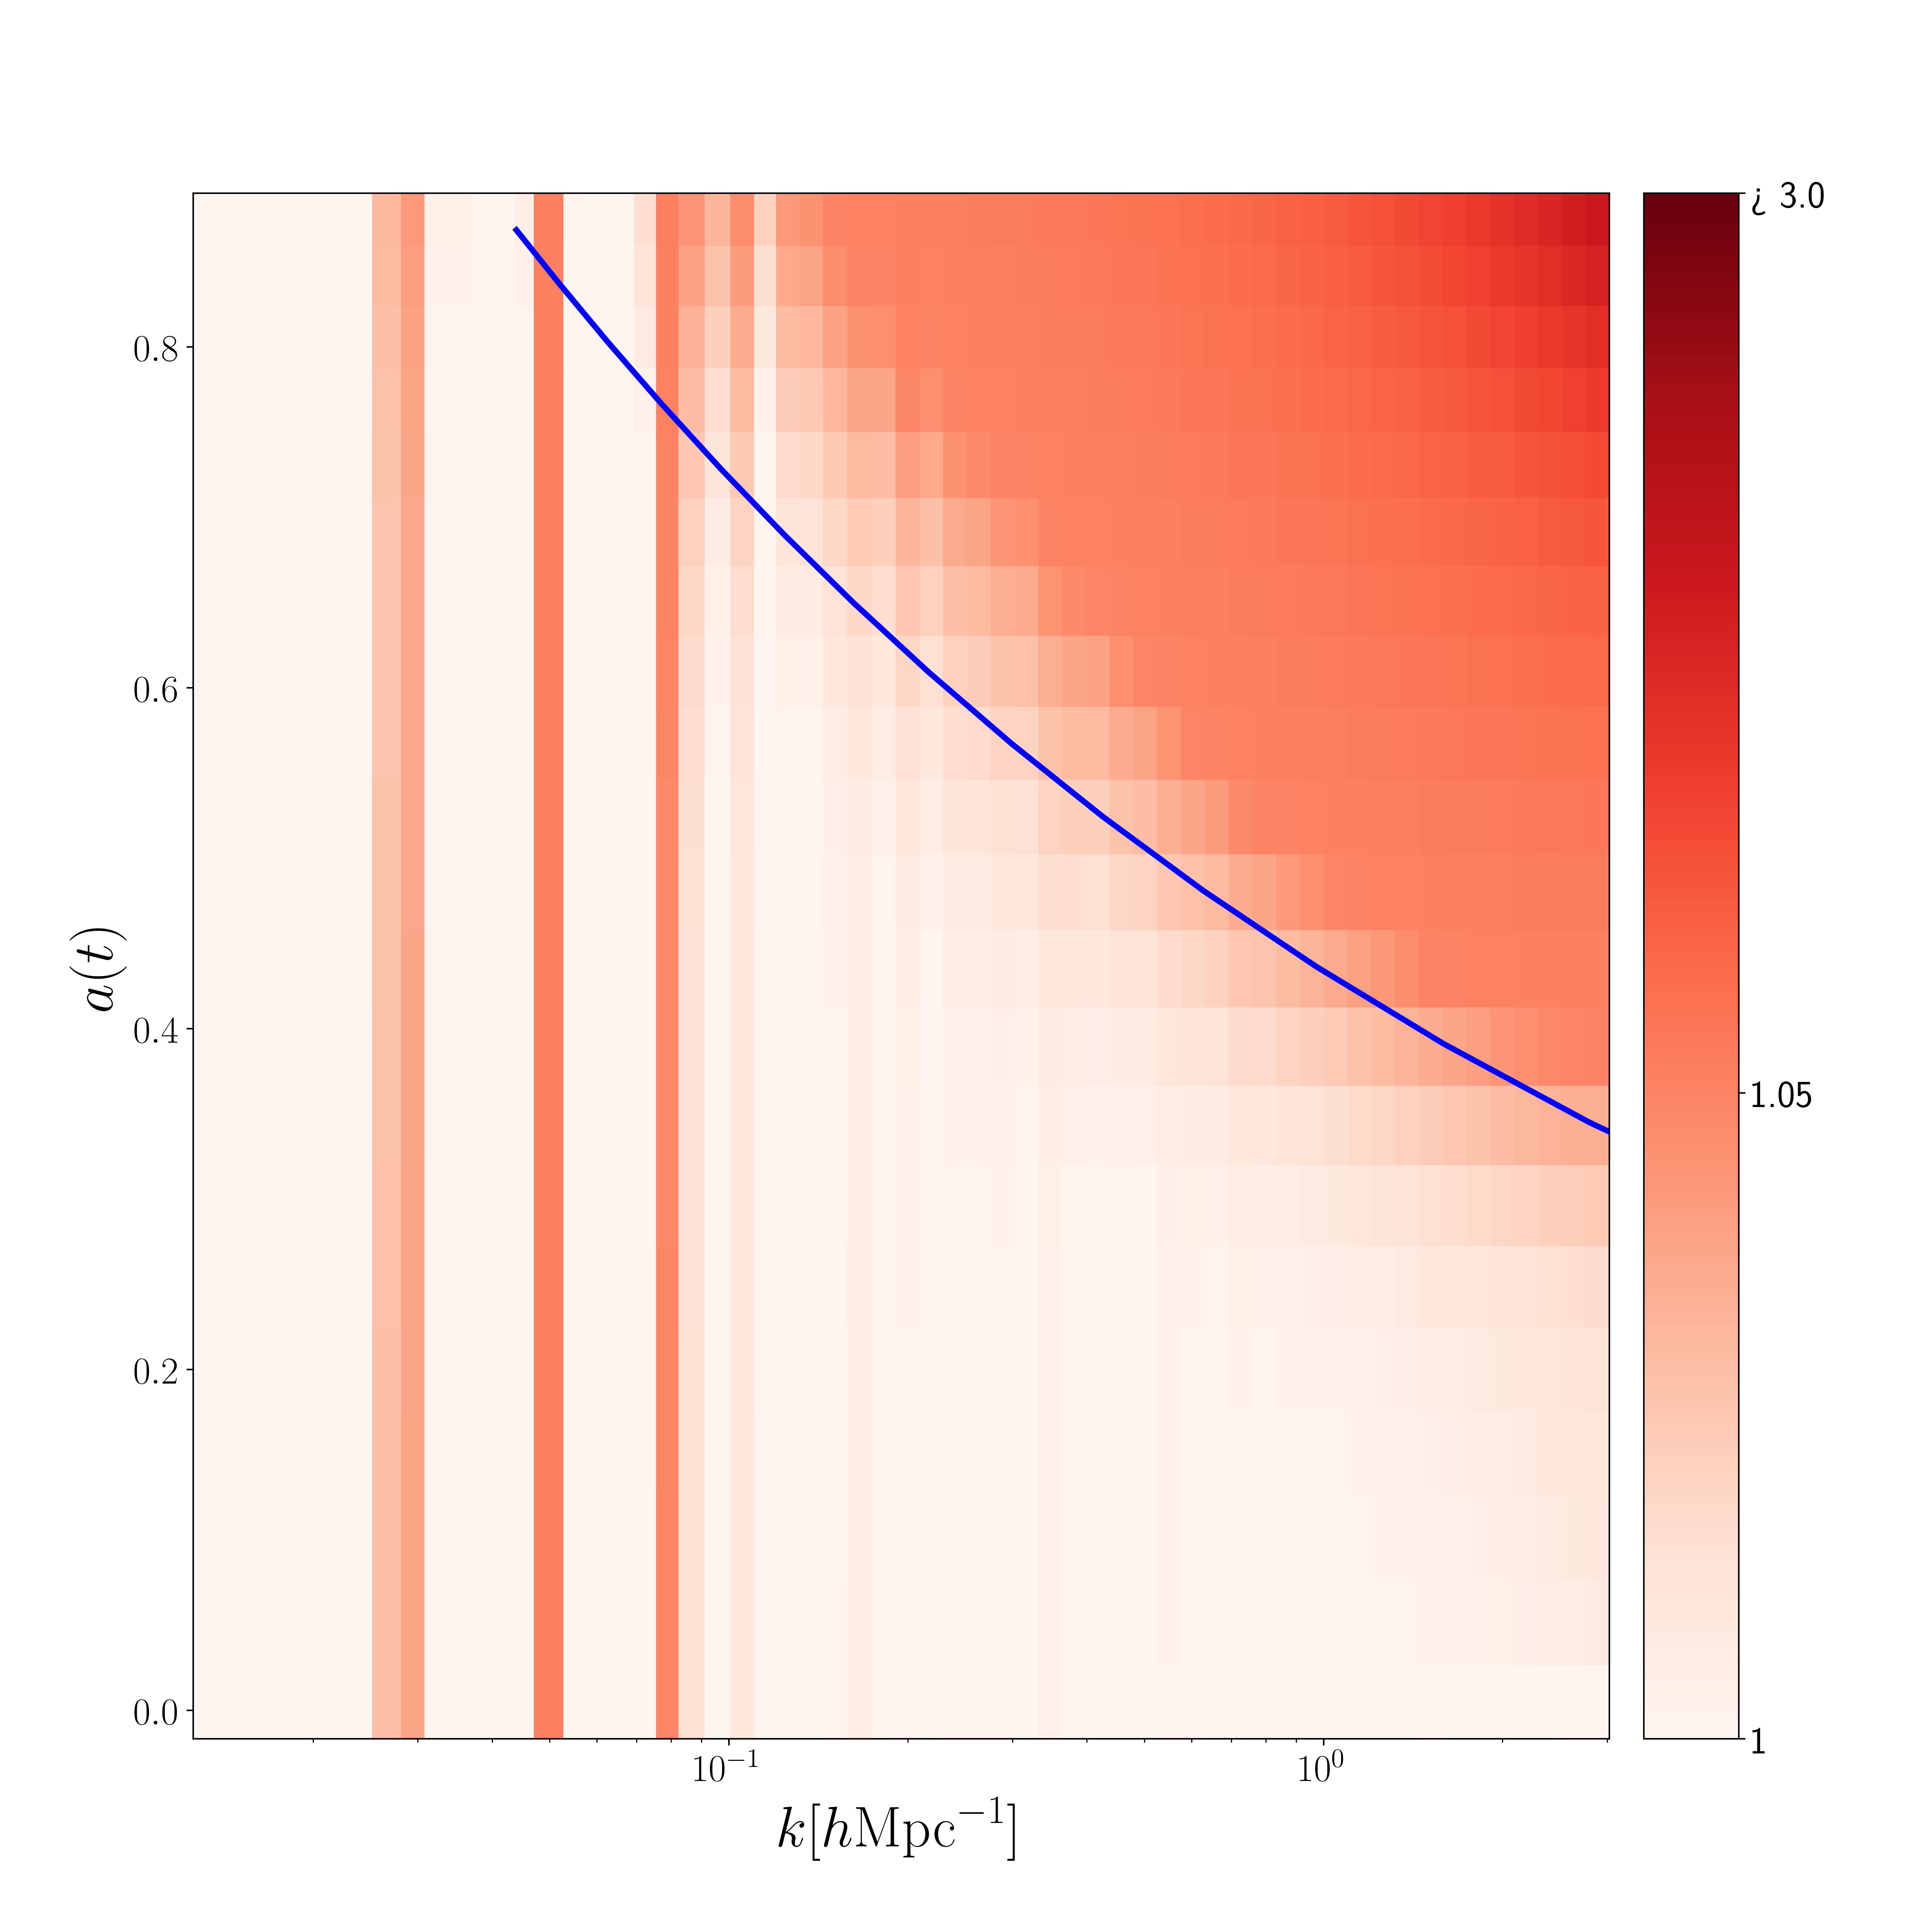
\includegraphics[width=1.0\linewidth]{simulations_approx/chi/chi_pwr_diff_map_512m_1p_1024M_500b_nl.png}
	\caption{Ratio of the FPA power spectrum in chameleon gravity $(n=0.5,\ \Phiscr=10^{-5})$ to the simulation run with standard gravity as function of time. Blue solid line is a chameleon mass \eqref{eq:chi_m}.}
	\label{fig:chi_pwr_diff_map}
\end{figure}

%%%%%%%%%%%%%%%%%%%%%%%%%%%%%%%%%%%%%%%%
% Correlation function
%%%%%%%%%%%%%%%%%%%%%%%%%%%%%%%%%%%%%%%%
\subsection{Correlation function}
In \autoref{fig:chi_corr_func}, we display the correlation function for one particular case of chameleon gravity -- $n=0.5,\ \Phiscr=10^{-5}$ at $z=0.5$. In \autoref{fig:chi_corr_peak}, we show the effects of different parameters of chameleon gravity through the BAO peak (amplitude, location and width). In this plot, the BAO peak characteristics are shown relative to the non-linear prediction (at the effective time) from the emulator. Comparison is done both for FPA (left) and FFA (right). We see that chameleon generally leads to a higher amplitude of the peak, a slight shift to the higher $r$ and a narrower width of the peak. All these effects are stronger for FFA than for FPA (as expected).

\begin{figure*}
\centering
	\begin{subfigure}{1.2\textwidth}
        \includegraphicscustomlegend{simulations_approx/chi/chi_corr_func_r2_z_z_eff}
	\end{subfigure}
	\begin{subfigure}{1.0\textwidth}
		\centering
		\includegraphicscustom{simulations_approx/chi/chi_corr_func_r2_z_z_eff}
	\end{subfigure}
	\begin{subfigure}{1.0\textwidth}
		\centering
		\includegraphicscustom{simulations_approx/chi/chi_ff_corr_func_r2_z_z_eff}
	\end{subfigure}
	\caption{Correlation function for chameleon gravity $(n=0.5,\ \Phiscr=10^{-5})$ at $z=0.5$. On the top are shown results using FPA whereas on the bottom using FFA}
	\label{fig:chi_corr_func}
\end{figure*}

\begin{figure*}
\centering
%%%%%%%%%%%%%%%%%%%%%%%%%%%%%%%%%%%%%
% Legend
%%%%%%%%%%%%%%%%%%%%%%%%%%%%%%%%%%%%%
	\begin{subfigure}{1.2\textwidth}
        \includegraphicscustomlegend{simulations_approx/chi/nl_fp_corr_peak_amp_z_eff}
	\end{subfigure}
%%%%%%%%%%%%%%%%%%%%%%%%%%%%%%%%%%%%%
% Amplitude
%%%%%%%%%%%%%%%%%%%%%%%%%%%%%%%%%%%%%
	\begin{subfigure}{0.5\textwidth}
		\includegraphicscustom{simulations_approx/chi/nl_fp_corr_peak_amp_z_eff}
		\caption{Amplitude}
	\end{subfigure}%
	\begin{subfigure}{0.5\textwidth}
		\includegraphicscustom{simulations_approx/chi/nl_ff_corr_peak_amp_z_eff}
		\caption{Amplitude}
	\end{subfigure}
%%%%%%%%%%%%%%%%%%%%%%%%%%%%%%%%%%%%%
% Loation
%%%%%%%%%%%%%%%%%%%%%%%%%%%%%%%%%%%%%
	\begin{subfigure}{0.5\textwidth}
		\includegraphicscustom{simulations_approx/chi/nl_fp_corr_peak_loc_z_eff}
		\caption{Location}
	\end{subfigure}%
	\begin{subfigure}{0.5\textwidth}
		\includegraphicscustom{simulations_approx/chi/nl_ff_corr_peak_loc_z_eff}
		\caption{Location}
	\end{subfigure}
%%%%%%%%%%%%%%%%%%%%%%%%%%%%%%%%%%%%%
% Width
%%%%%%%%%%%%%%%%%%%%%%%%%%%%%%%%%%%%%
	\begin{subfigure}{0.5\textwidth}
		\includegraphicscustom{simulations_approx/chi/nl_fp_corr_peak_width_z_eff}
		\caption{Width}
	\end{subfigure}%
	\begin{subfigure}{0.5\textwidth}
		\includegraphicscustom{simulations_approx/chi/nl_ff_corr_peak_width_z_eff}
		\caption{Width}
	\end{subfigure}
%%%%%%%%%%%%%%%%%%%%%%%%%%%%%%%%%%%%%
% Caption
%%%%%%%%%%%%%%%%%%%%%%%%%%%%%%%%%%%%%
	\caption{Location, amplitude and width of the BAO peak as a function of the redshift for different values of chameleon parameters. On the left, the characteristics are shown for simulations using FPA, while on the right, for simulations using FFA.}
	\label{fig:chi_corr_peak}
\end{figure*}

%%%%%%%%%%%%%%%%%%%%%%%%%%%%%%%%%%%%%%%%
% Halo mass function
%%%%%%%%%%%%%%%%%%%%%%%%%%%%%%%%%%%%%%%%
\subsection{Halo mass function}
In \autoref{fig:chi_diff_hmf} we compared the (relative) halo mass function for different parameters of chameleon gravity. We see that in the mass range $(10^{12}--10^{14}M_\odot)$ all the simulations give very similar results and differ more outside this range. We see that higher the screening potential $\Phiscr$ the more power on small scales and therefore more massive halos. For distinguishing between different chameleon parameters we should therefore use the most massive halos $(M\gtrsim10^{14}M_\odot)$.
\begin{figure*}
	\centering
		\begin{subfigure}{1.2\textwidth}
			\includegraphicscustomlegend{simulations_approx/chi/hmf_z0.5_b500_M512_chi_hmf_z_z_eff}
		\end{subfigure}
		\begin{subfigure}{1.0\textwidth}
			\centering
			\includegraphicscustom{simulations_approx/chi/hmf_z0.5_b500_M512_chi_hmf_z_z_eff}
		\end{subfigure}
		\caption{Halo mass function (relative) for non-linear chameleon gravity with different chameleon parameters.}
		\label{fig:chi_diff_hmf}
	\end{figure*}